\documentclass{article}
\usepackage[utf8]{inputenc}

\documentclass[a4paper]{article}
\usepackage[12pt]{extsizes}
\usepackage{amsmath,amsthm,amssymb}
\usepackage[hidelinks]{hyperref} 
\usepackage[warn]{mathtext}
\usepackage[T1,T2A]{fontenc}
\usepackage[utf8]{inputenc}
\usepackage[english,russian]{babel}
\usepackage{tocloft}
\linespread{1.5}
\usepackage{indentfirst}
\usepackage{setspace}
%\полуторный интервал
\onehalfspacing

\newcommand{\RomanNumeralCaps}[1]
    {\MakeUppercase{\romannumeral #1}}

\usepackage{amssymb}

\usepackage{graphicx, float}
\graphicspath{{pictures/}}
\DeclareGraphicsExtensions{.pdf,.png,.jpg}
\usepackage[left=25mm,right=1cm,
    top=2cm,bottom=20mm,bindingoffset=0cm]{geometry}
\renewcommand{\cftsecleader}{\cftdotfill{\cftdotsep}}

\addto\captionsrussian{\renewcommand{\contentsname}{СОДЕРЖАНИЕ}}
\addto\captionsrussian{\renewcommand{\listfigurename}{СПИСОК ИЛЛЮСТРАЦИЙ}}

\usepackage{fancyhdr}
\usepackage[nottoc]{tocbibind}

\fancypagestyle{plain}{
\fancyhf{}
\renewcommand{\headrulewidth}{0pt}
\fancyhead[R]{\thepage}
}

\usepackage{blindtext}
\pagestyle{myheadings}
\usepackage{hyperref}

\begin{document}
\begin{titlepage}
  \begin{center}
    \large
    Санкт-Петербургский политехнический университет Петра Великого
    
    Институт прикладной математики и механики
    
    \textbf{Высшая школа прикладной математики и вычислительной физики}
    \vfill
    \textsc{\textbf{\Large{Отчёт по лабораторной работе №4}}}\\[5mm]
    \\ по дисциплине
    \\ <<Математическая статистика>>\\
\end{center}

\vfill

\begin{tabular}{l p{140} l}
Выполнила студентка \\группы 3630102/80401 && Мамаева Анастасия Сергеевна \\
\\
Проверил\\Доцент, к.ф.-м.н.& \hspace{0pt} &   Баженов Александр Николаевич \\\\
\end{tabular}

\hfill \break
\hfill \break
\begin{center} Санкт-Петербург \\2021 \end{center}
\thispagestyle{empty}
\end{titlepage}
\newpage
\newpage
\begin{center}
    \setcounter{page}{2}
    \tableofcontents
\end{center}
\newpage
\begin{center}
    \setcounter{page}{3}
    \listoffigures
\end{center}

\newpage

\section {Постановка задачи}
\noindent Сгенерировать выборки размером 20, 60 и 100 элементов. Построить на них эмпирические функции распределения и ядерные оценки плотности распределения на отрезке $[-4;\,4]$ для непрерывных распределений и на отрезке $[6;\,14]$ для распределения Пуассона.

\section {Теория}
\subsection{Эмпирическая функция распределения}
\subsubsection{Статистический ряд}
\noindent Статистическим рядом назовем совокупность, состоящую из последовательности $\displaystyle\{z_i\}_{i=1}^k$ попарно различных элементов выборки, расположенных по возрастанию, и последовательности $\displaystyle\{n_i\}_{i=1}^k$ частот, с которыми эти элементы содержатся в выборке.
\subsubsection{Эмпирическая функция распределения}
\noindent Эмпирическая функция распределения (э. ф. р.) - относительная частота события $X < x$, полученная по данной выборке:
\begin{equation}
    F_n^*(x)=P^*(X<x).
\end{equation}
\subsubsection{Нахождение э. ф. р.}
\begin{equation}
    F^*(x)=\frac{1}{n}\sum_{z_i<x}n_i.
\end{equation}
$F^*(x)-$ функция распределения дискретной случайной величины $X^*$, заданной таблицей распределения
\begin{table}[H]
    \centering
    \begin{tabular}{|c|c|c|c|c|}
        \hline
         $X^*$&$z_1$&$z_2$&...&$z_k$\\
         \hline
         $P$&$n_1/n$&$n_2/n$&...&$n_k/n$\\
         \hline
    \end{tabular}
    \caption{Таблица распределения}
    \label{tab:my_label}
\end{table}
\noindent Эмпирическая функция распределения является оценкой, т. е. приближённым значением, генеральной функции распределения
\begin{equation}
    F_n^*(x)\approx F_X(x).
\end{equation}
\subsection{Оценки плотности вероятности}
\subsubsection{Определение}
\noindent Оценкой плотности вероятности $f(x)$ называется функция $\widehat{f}(x)$, построенная на основе выборки, приближённо равная $f(x)$
\begin{equation}
    \widehat{f}(x)\approx f(x).
\end{equation}
\subsubsection{Ядерные оценки}
\noindent Представим оценку в виде суммы с числом слагаемых, равным объёму выборки:
\begin{equation}
    \widehat{f}_n(x)=\frac{1}{n h_n}\sum_{i=1}^n K\left(\frac{x-x_i}{h_n}\right).
\end{equation}
$K(u)$ - ядро, т. е. непрерывная функция, являющаяся плотностью вероятности, $x_1,...,x_n$ $-$ элементы выборки, а $\{h_n\}_{n\in\mathbb{N}}$ - последовательность элементов из $\mathbb{R}_+$ такая, что
\begin{equation}
    h_n\xrightarrow[n\to\infty]{}0;\;\;\;n h_n\xrightarrow[n\to\infty]{}\infty.
\end{equation}
Такие оценки называются непрерывными ядерными.\\\\
Гауссово ядро:
\begin{equation}
    K(u)=\frac{1}{\sqrt{2\pi}}e^{-\frac{u^2}{2}}.
\end{equation}
Правило Сильвермана:
\begin{equation}
    h_n=\left(\frac{4\hat{\sigma}^5}{3n}\right)^{1/5}\approx1.06\hat{\sigma}n^{-1/5},
\end{equation}
где $\hat{\sigma}$ - выборочное стандартное отклонение.

\section {Программная реализация} 	
\noindent Лабораторная работа выполнена на языке Python вресии 3.7 в среде разработки JupyterLab. Использовались дополнительные библиотеки:
 \begin{enumerate}
        \item scipy (генерация выборок)
        \item statsmodels (построение эмпирических функций распределения)
        \item matplotlib, seaborn (визуализация)
        \item numpy (вычисление ряда числовых характеристик)
    \end{enumerate}
В приложении находится ссылка на GitHub репозиторий с исходныи кодом.

\section {Результаты} 

\subsection{Эмпирическая функция распределения}
	\begin{figure}[H]
	\centering
	{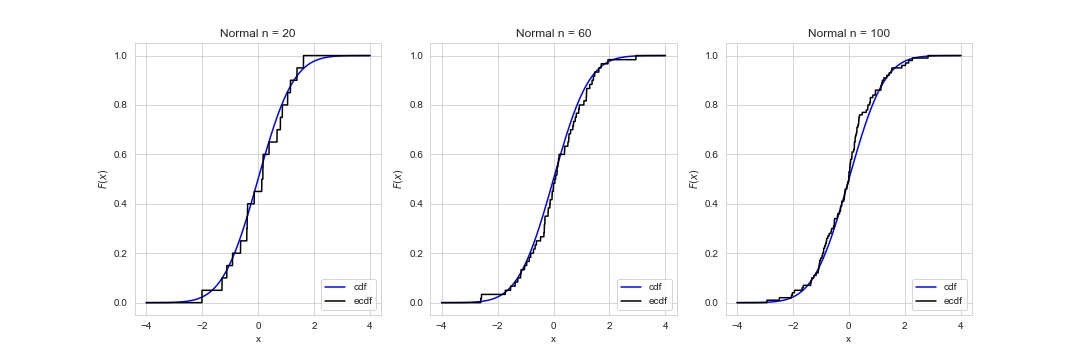
\includegraphics[scale=0.51]{Normal100.pdf}}
		\caption{нормальное распределение} 
		\label{fig:normal}
	\end{figure}

\begin{figure}[H]
	{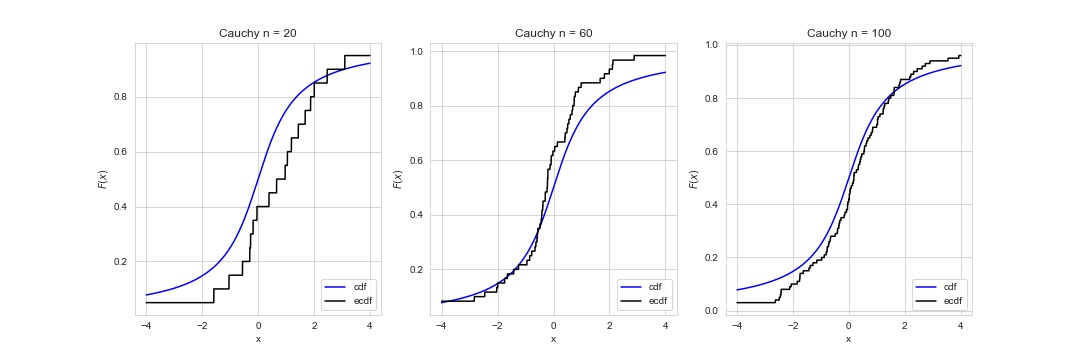
\includegraphics[scale=0.51]{Cauchy100.pdf}}
		\caption{распределение Коши} 
		\label{fig:normal}
	\end{figure}

\begin{figure}[H]
	{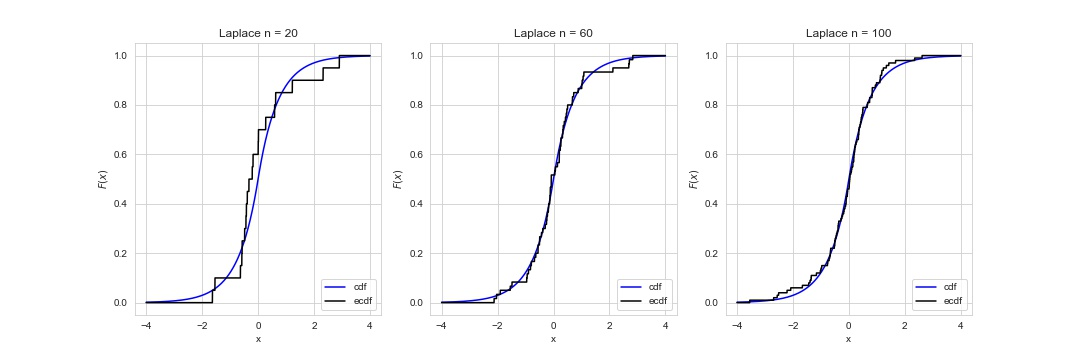
\includegraphics[scale=0.51]{Laplace100.pdf}}
		\caption{распределение Лапласа} 
		\label{fig:normal}
	\end{figure}
	
\begin{figure}[H]
	{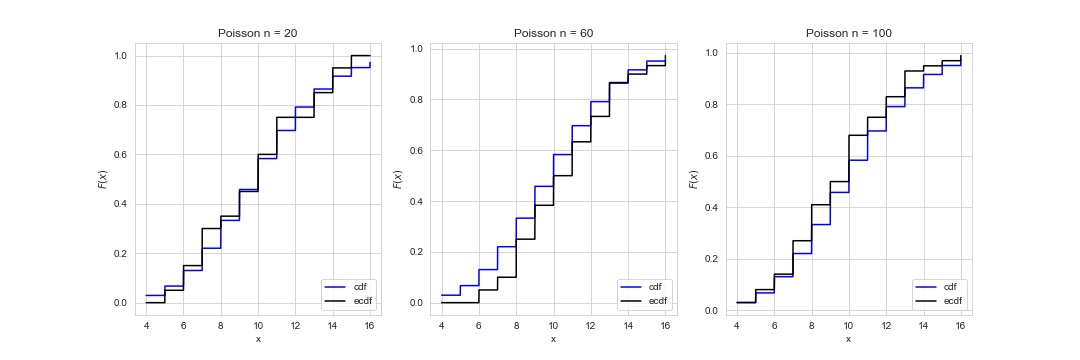
\includegraphics[scale=0.51]{Poisson100.pdf}}
		\caption{распределение Пуассона} 
		\label{fig:normal}
	\end{figure}
	
\begin{figure}[H]
	{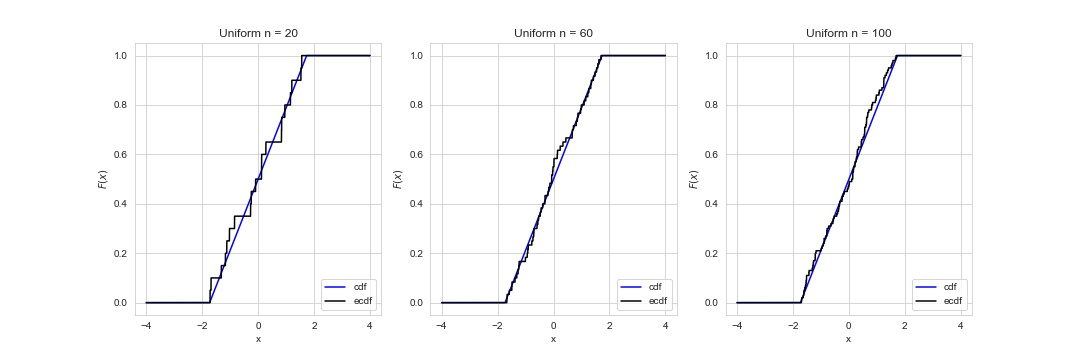
\includegraphics[scale=0.51]{Uniform100.pdf}}
		\caption{равномерное распределение} 
		\label{fig:normal}
	\end{figure}
	
\subsection{Ядерные оценки плотности распределения}
\begin{figure}[H]
	{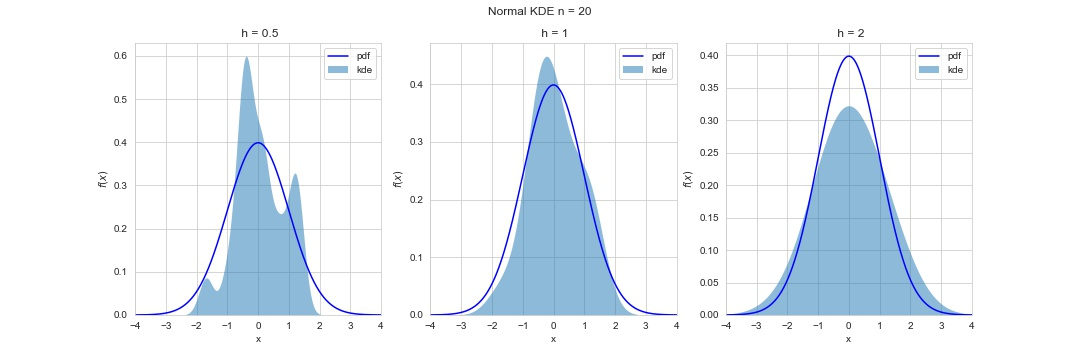
\includegraphics[scale=0.51]{NormalKDE20.pdf}}
		\caption{нормальное распределение, $n=20$} 
		\label{fig:normal}
	\end{figure}
	
\begin{figure}[H]
	{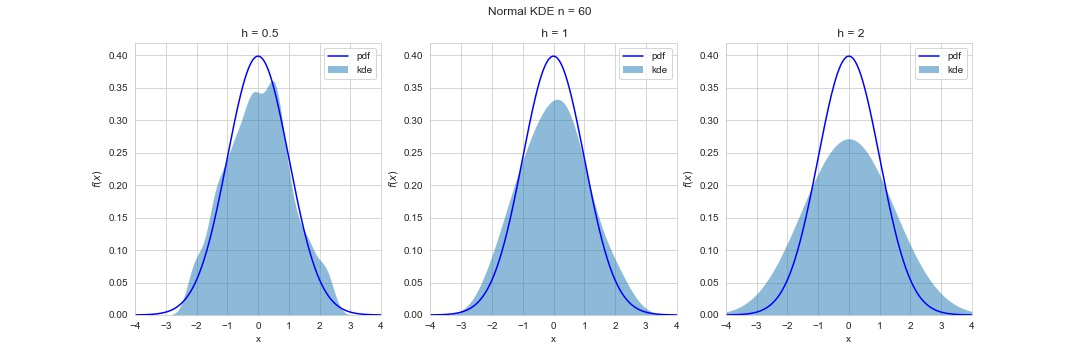
\includegraphics[scale=0.51]{NormalKDE60.pdf}}
		\caption{нормальное распределение, $n=60$} 
		\label{fig:normal}
	\end{figure}
		
\begin{figure}[H]
	{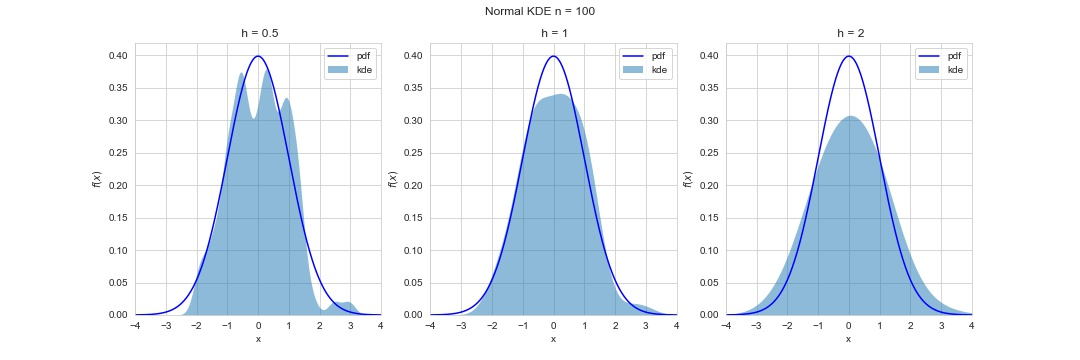
\includegraphics[scale=0.51]{NormalKDE100.pdf}}
		\caption{нормальное распределение, $n=100$} 
		\label{fig:normal}
	\end{figure}

\begin{figure}[H]
	{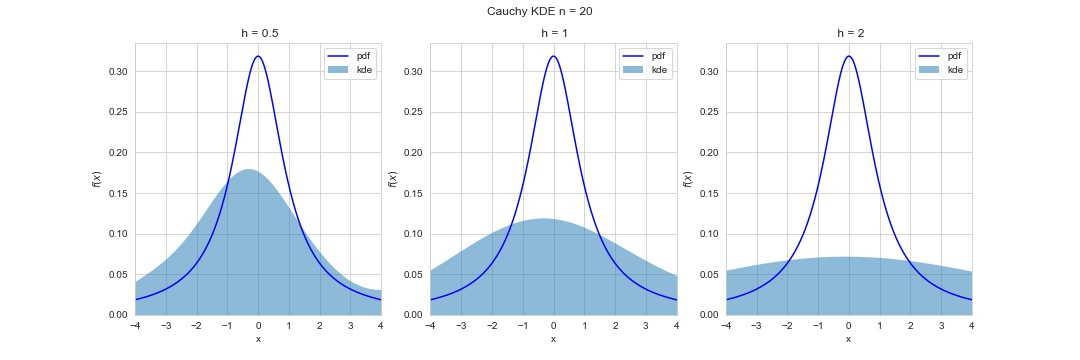
\includegraphics[scale=0.51]{CauchyKDE20.pdf}}
		\caption{распределение Коши, $n=20$} 
		\label{fig:normal}
	\end{figure}
	
\begin{figure}[H]
	{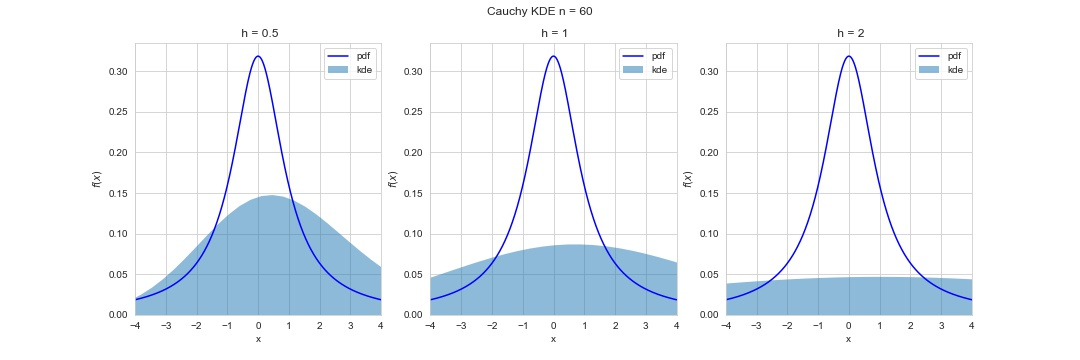
\includegraphics[scale=0.51]{CauchyKDE60.pdf}}
		\caption{распределение Коши, $n=60$} 
		\label{fig:normal}
	\end{figure}
	
\begin{figure}[H]
	{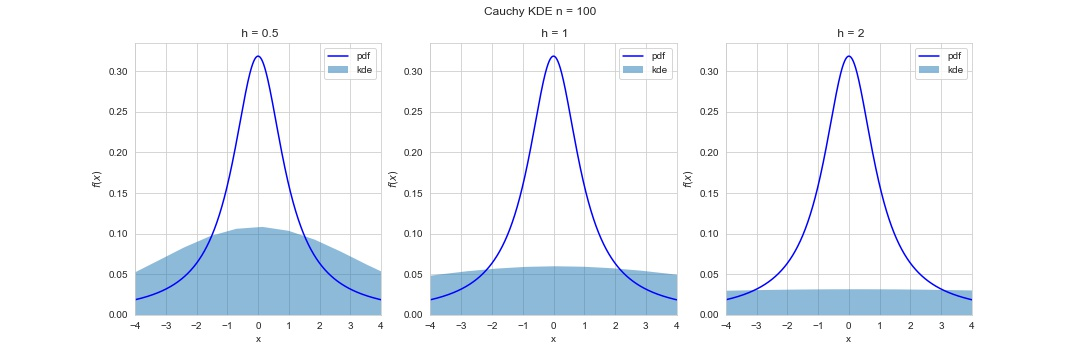
\includegraphics[scale=0.51]{CauchyKDE100.pdf}}
		\caption{распределение Коши, $n=100$} 
		\label{fig:normal}
	\end{figure}
	
\begin{figure}[H]
	{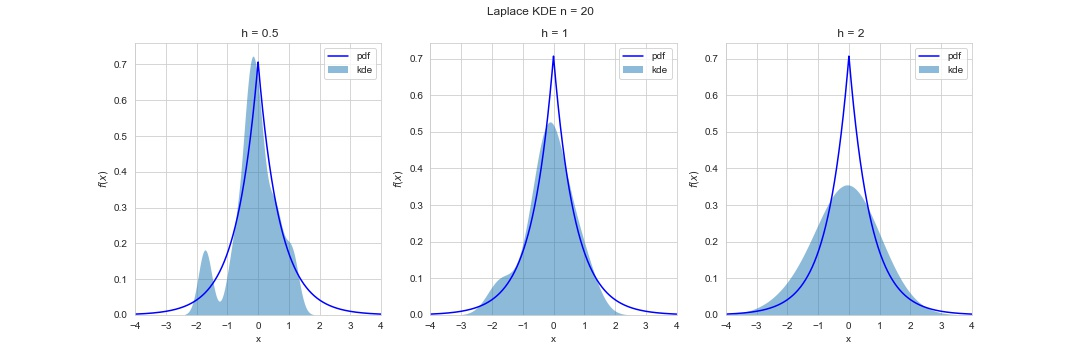
\includegraphics[scale=0.51]{LaplaceKDE20.pdf}}
		\caption{распределение Лапласа, $n=20$} 
		\label{fig:normal}
	\end{figure}

\begin{figure}[H]
	{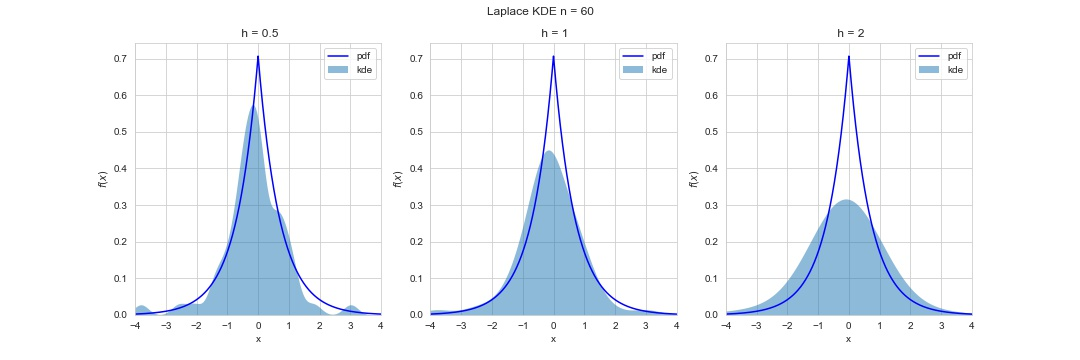
\includegraphics[scale=0.51]{LaplaceKDE60.pdf}}
		\caption{распределение Лапласа, $n=60$} 
		\label{fig:normal}
	\end{figure}
		
\begin{figure}[H]
	{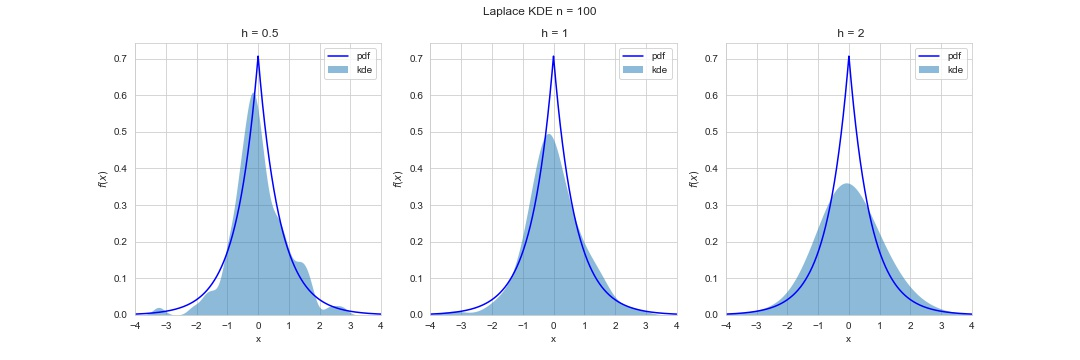
\includegraphics[scale=0.51]{LaplaceKDE100.pdf}}
		\caption{распределение Лапласа, $n=100$} 
		\label{fig:normal}
	\end{figure}
		
\begin{figure}[H]
	{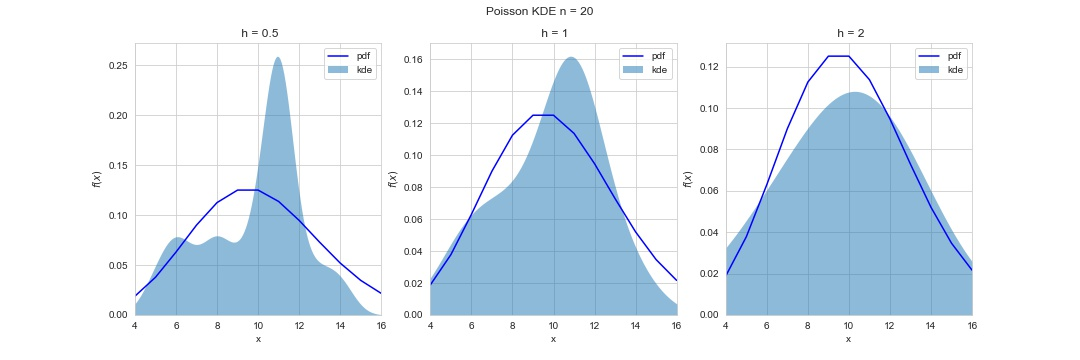
\includegraphics[scale=0.51]{PoissonKDE20.pdf}}
		\caption{распределение Пуассона, $n=20$} 
		\label{fig:normal}
	\end{figure}
	
\begin{figure}[H]
	{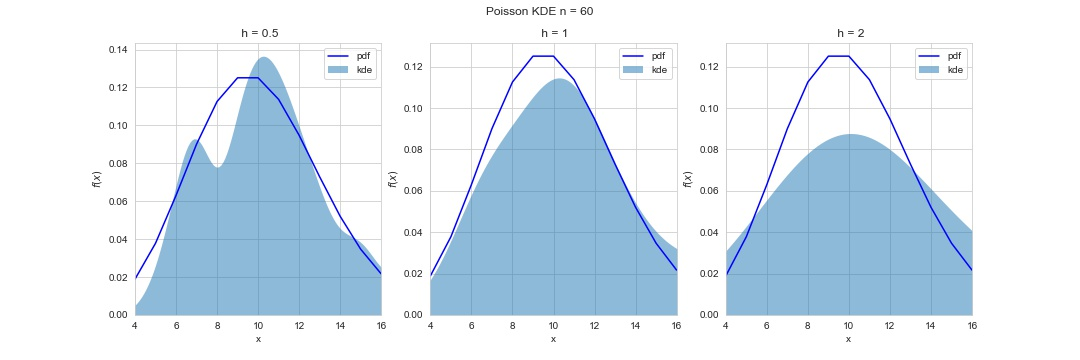
\includegraphics[scale=0.51]{PoissonKDE60.pdf}}
		\caption{распределение Пуассона, $n=60$} 
		\label{fig:normal}
	\end{figure}
	
\begin{figure}[H]
	{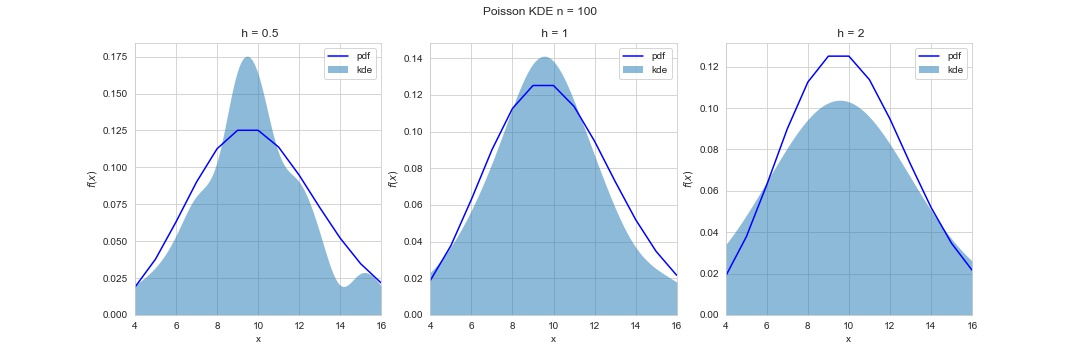
\includegraphics[scale=0.51]{PoissonKDE100.pdf}}
		\caption{распределение Пуассона, $n=100$} 
		\label{fig:normal}
	\end{figure}
	
\begin{figure}[H]
	{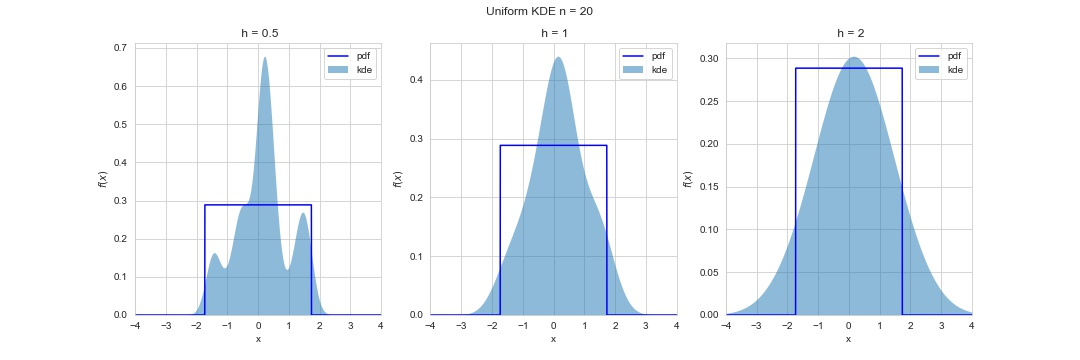
\includegraphics[scale=0.51]{UniformKDE20.pdf}}
		\caption{равномерное распределение, $n=20$} 
		\label{fig:normal}
	\end{figure}
	
\begin{figure}[H]
	{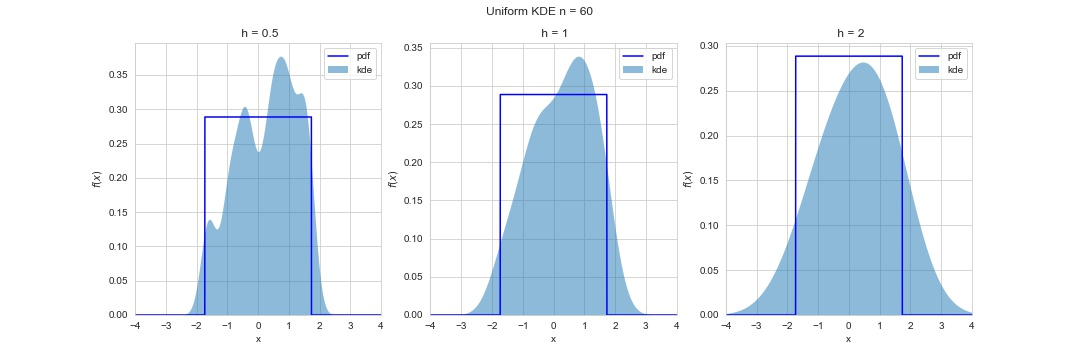
\includegraphics[scale=0.51]{UniformKDE60.pdf}}
		\caption{равномерное распределение, $n=60$} 
		\label{fig:normal}
	\end{figure}

\begin{figure}[H]
	{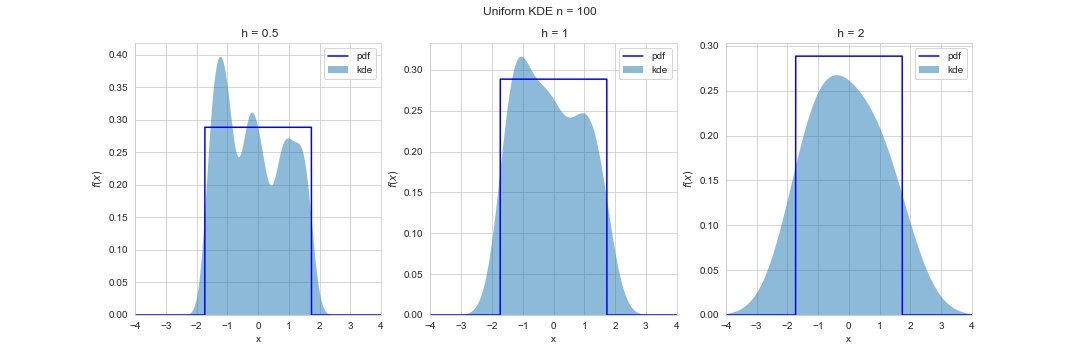
\includegraphics[scale=0.51]{UniformKDE100.pdf}}
		\caption{равномерное распределение, $n=100$} 
		\label{fig:normal}
	\end{figure}
	
\section{Обсуждение}
\noindent Можем наблюдать на иллюстрациях с эмпирическими функциями, что ступенчатая эмпирическая функция распределения тем лучше приближает функцию распределения реальной выборки, чем мощнее эта выборка. Заметим так же, что для распределения Пуассона и равномерного распределения отклонение функций друг от друга наибольшее.\\\\
\noindent Рисунки, посвященные ядерным оценкам, иллюстрируют сближение ядерной оценки и функции плотности вероятности для всех $h$ с ростом размера выборки. Для распределения Пуассона наиболее ярко видно, как сглаживает отклонения увеличение параметра сглаживания $h$.\\\\
\noindent В зависимости от особенностей распределений для их описания лучше подходят разные параметры $h$ в ядерной оценке: для нормального, равномерного и пуассоновского распределений оптимальным значением параметра является $h=h_n$, а для распределений Коши и Лапласса - $h=h_n/2$.\\\\
\noindent Также можно увидеть, что чем больше коэффициент при параметре сглаживания $\hat{h_n}$, тем меньше изменений знака производной у аппроксимирующей функции, вплоть до того, что при $h=h_n/2$ функция становится унимодальной на рассматриваемом промежутке. Также видно, что при $h=h_n/2$ по полученным приближениям становится сложно сказать плотность вероятности какого распределения они должны повторять, так как они очень похожи между собой.

\section{Приложение}

\noindent Код программы GitHub URL:\\
\newline https://github.com/Brightest-Sunshine/Math-Statistic-2021/blob/main/Lab4/Lab4.ipynb

\end{document}
